\documentclass{../vespers-booklet}
\usepackage{multicol}

\begin{document}

% TODO: Update the title for the specific feast
\chapter*{Second Vespers of the Feast of the Most Holy Rosary}

%\section*{Beginning of the Office}

\begin{center}
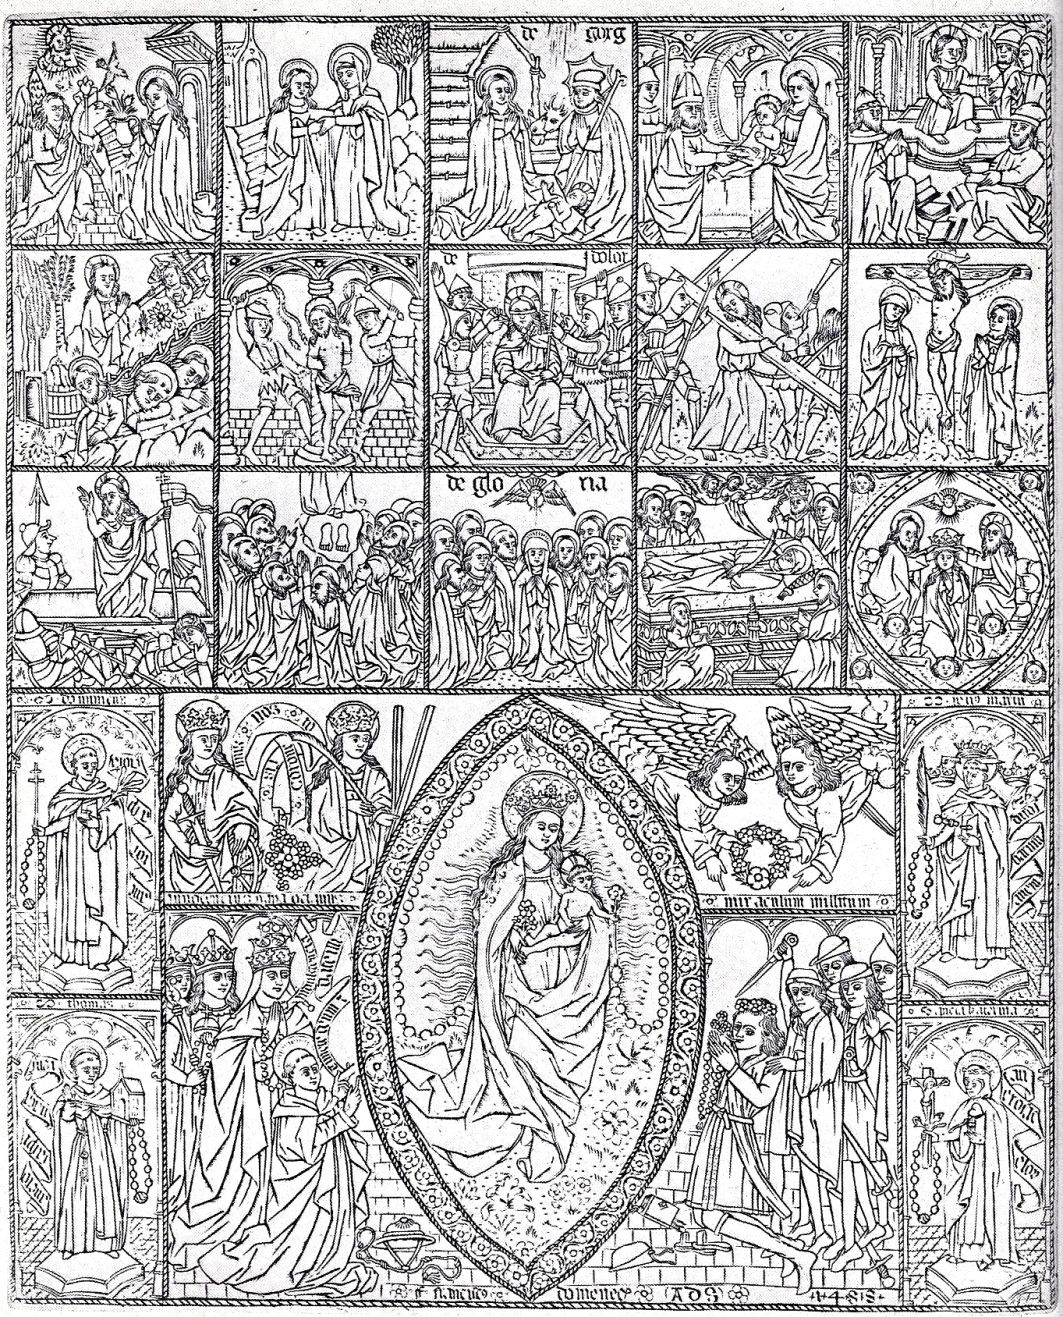
\includegraphics[width=0.8\textwidth]{HolyRosary}
\end{center}

\vfill\pagebreak

\begin{rubricbox}

{\color{red}When the Officiant kneels, all \textbf{kneel} and pray silently.
Then, when the Officiant stands, all \textbf{stand} and say silently one \textit{Pater noster} (Our Father) and \textit{Ave Maria} (Hail Mary).
Then all make the sign of the cross with the Officiant as he intones:}

\end{rubricbox}

% TODO: Make sure that the tone of the deus adjutorium matches the season primarily and the solemnity of the feast secondarily
 \gresetinitiallines{1}
\gregorioscore{../common/deus-in-adjutorium-solemn}

\textit{
O God, come to my assistance.
{\color{red}\Rbar.}~O Lord, make haste to help me.
Glory be to the Father, and to the Son, and to the Holy Spirit,
as it was in the beginning, is now, and ever shall be, world without end. Amen.
Praise to Thee, O Lord, King of endless glory.}

\vfill\pagebreak

%TODO: Add that the correct psalms, and verify that their tones, and their associated pointed text are correct

\section*{Psalm 109}

\textit{\textnormal{Ant. 1.} Who is this, * fair as a dove, like a rose-tree planted beside the rivers of waters?
 \textnormal{Ps.} The Lord said to my Lord: * Sit thou at my right hand.}
 
 \begin{rubricbox}

{\color{red}All remain standing throughout the first antiphon.
After the psalm is intoned by the Cantor, all \textbf{sit} at the asterisk.}

\end{rubricbox}

\gresetinitiallines{1}
\gregorioscore{ps109-antiphon}

\gresetinitiallines{0}
\gregorioscore{ps109-intonation}

 \begin{latinenglishsection}

\latinenglish{

	 2. Donec ponam inimícos \textbf{tu}os,~*
	scabéllum pe\textit{dum} \textit{tu}\textbf{ó}rum.
	
3. Virgam virtútis tuæ emíttet Dóminus ex \textbf{Si}on:~*
	domináre in médio inimicó\textit{rum} \textit{tu}\textbf{ó}rum.
	
4. Tecum princípium in die virtútis tuæ in splendóribus sanc\textbf{tó}rum:~*
	ex útero ante lucíferum \textit{gé}\textit{nu}\textbf{i} te.
	
5. Jurávit Dóminus, et non p{\oe}nitébit \textbf{e}um:~*
	Tu es sacérdos in ætérnum secúndum órdi\textit{nem} \textit{Mel}\textbf{chí}se\-dech.
	
6. Dóminus a dextris \textbf{tu}is,~* 
	confrégit in die iræ \textit{su}\textit{æ} \textbf{re}ges.
	
7. Judicábit in natiónibus, implébit ru\textbf{í}nas:~*
	conquassábit cápita in ter\textit{ra} \textit{mul}\textbf{tó}rum.
	
8. De torrénte in via \textbf{bi}bet:~* {\color{red}\textit{(stand)}}
	proptérea exal\textit{tá}\textit{bit} \textbf{ca}put.

{\color{red}\textit{(bow)}} Glória Patri, et \textbf{Fí}lio,~*
	et Spirí\textit{tu}\textit{i} \textbf{Sanc}to.
	
{\color{red}\textit{(rise)}} Sicut erat in princípio, et nunc, et \textbf{sem}per,~*
	et in s\'{\ae}cula sæcu\textit{ló}\textit{rum}. \textbf{A}men. %%

}{
	% 1. The Lord said to my Lord: Sit thou at my right hand:

2. Until I make thy enemies thy footstool.
 
3. The Lord will send forth the sceptre of thy power out of Sion: rule thou in the midst of thy enemies.
 
4. With thee is the principality in the day of thy strength: in the brightness of the saints:
 from the womb before the day star I begot thee.
 
5. The Lord hath sworn, and he will not repent: Thou art a priest for ever according to the order of Melchisedech.
 
6. The Lord at thy right hand hath broken kings in the day of his wrath.

7. He shall judge among nations, he shall fill ruins: he shall crush the heads in the land of the many.

8. He shall drink of the torrent in the way: therefore shall he lift up the head. 

Glory be. %%
}

\end{latinenglishsection}

\gresetinitiallines{1}
\gregorioscore{ps109-antiphon}

%%

\section*{Psalm 112}

\textit{\textnormal{Ant. 2.} A virgin most mighty, * like the tower of David, whereon there hung a thousand bucklers, all the shields of valiant men.
 \textnormal{Ps.} Praise the Lord, ye children: * praise ye the name of the Lord.}

 \begin{rubricbox}

{\color{red}The remaining Psalms are said in the same manner as the first.}

\end{rubricbox}

\gresetinitiallines{1}
\gregorioscore{ps112-antiphon}

\gresetinitiallines{0}
\gregorioscore{ps112-intonation}

 \begin{latinenglishsection}

\latinenglish{

	2. Sit nomen Dómi\textit{ni} \textit{be}\textit{ne}\textbf{díc}tum,~* 
	ex hoc nunc, et us\textit{que} \textit{in} \textbf{s\'{\ae}}culum.

3. A solis ortu us\textit{que} \textit{ad} \textit{oc}\textbf{cá}sum,~* 
	laudábile \textit{no}\textit{men} \textbf{Dó}mini.

4. Excélsus super om\textit{nes} \textit{gen}\textit{tes} \textbf{Dó}\textbf{mi}nus,~* 
	et super cælos gló\textit{ri}\textit{a} \textbf{e}jus.

5. Quis sicut Dóminus, Deus noster, qui \textit{in} \textit{al}\textit{tis} \textbf{há}\textbf{bi}tat,~* 
	et humília réspicit in cælo \textit{et} \textit{in} \textbf{ter}ra?

6. Súscitans \textit{a} \textit{ter}\textit{ra} \textbf{ín}\textbf{o}pem,~* 
	et de stércore é\textit{ri}\textit{gens} \textbf{páu}perem:

7. Ut cóllocet e\textit{um} \textit{cum} \textit{prin}\textbf{cí}\textbf{pi}bus,~* 
	cum princípibus pó\textit{pu}\textit{li} \textbf{su}i.

8. Qui habitáre facit sté\textit{ri}\textit{lem} \textit{in} \textbf{do}mo,~* 
	matrem filió\textit{rum} \textit{læ}\textbf{tán}tem.

9. {\color{red}\textit{(bow)}} Glória \textit{Pa}\textit{tri}, \textit{et} \textbf{Fí}\textbf{li}o,~* 
	et Spirí\textit{tu}\textit{i} \textbf{Sanc}to.

10. {\color{red}\textit{(rise)}}  Sicut erat in princípio, \textit{et} \textit{nunc}, \textit{et} \textbf{sem}per,~* 
	et in s\'{\ae}cula sæcu\textit{ló}\textit{rum}. \textbf{A}men. %%

}{
	%1. Praise the Lord, ye children: praise ye the name of the Lord.
 	
2. Blessed be the name of the Lord, from henceforth now and for ever.
 	
3. From the rising of the sun unto the going down of the same, the name of the Lord is worthy of praise.
 	
4. The Lord is high above all nations; and his glory above the heavens.
 	
5.Who is as the Lord our God, who dwelleth on high, and looketh down on the low things in heaven and in earth?
 	
6. Raising up the needy from the earth, and lifting up the poor out of the dunghill:
 	
7. That he may place him with princes, with the princes of his people.
 	
8. Who maketh a barren woman to dwell in a house, the joyful mother of children. 

Glory be. %%
}

\end{latinenglishsection}

\gresetinitiallines{1}
\gregorioscore{ps112-antiphon}

%%

\section*{Psalm 121}

\textit{\textnormal{Ant. 3.} Hail Mary, * full of grace, the Lord is with thee, blessed art thou among women.
 \textnormal{Ps.} I rejoiced at the things that were said to me: * We shall go into the house of the Lord.}

\gresetinitiallines{1}
\gregorioscore{ps121-antiphon}

\gresetinitiallines{0}
\gregorioscore{ps121-intonation}

 \begin{latinenglishsection}

\latinenglish{

	2. Stantes e\textit{rant} \textit{pe}\textit{des} \textbf{nos}tri,~* 
	in átriis tu\textit{is}, \textit{Je}\textbf{rú}salem.

3. Jerúsalem, quæ ædifi\textit{cá}\textit{tur} \textit{ut} \textbf{cí}\textbf{vi}tas:~* 
	cujus participátio ejus \textit{in} \textit{id}\textbf{íp}sum.

4. Illuc enim ascendérunt tri\textit{bus}, \textit{tri}\textit{bus} \textbf{Dó}\textbf{mi}ni:~* 
	testimónium Israël ad confiténdum nó\textit{mi}\textit{ni} \textbf{Dó}mini.

5. Quia illic sedérunt se\textit{des} \textit{in} \textit{ju}\textbf{dí}\textbf{ci}o,~* 
	sedes super \textit{do}\textit{mum} \textbf{Da}vid.

6. Rogáte quæ ad pa\textit{cem} \textit{sunt} \textit{Je}\textbf{rú}\textbf{sa}lem:~* 
	et abundántia\\ dili\textit{gén}\textit{ti}\textbf{bus} te:

7. Fiat pax in \textit{vir}\textit{tú}\textit{te} \textbf{tu}a:~* 
	et abundántia in túr\textit{ri}\textit{bus} \textbf{tu}is.

8. Propter fratres meos, et \textit{pró}\textit{xi}\textit{mos} \textbf{me}os,~* 
	loquébar \textit{pa}\textit{cem} \textbf{de} te:

9. Propter domum Dómi\textit{ni}, \textit{De}\textit{i} \textbf{nos}tri,~* 
	quæsívi \textit{bo}\textit{na} \textbf{ti}bi.

10. {\color{red}\textit{(bow)}} Glória \textit{Pa}\textit{tri}, \textit{et} \textbf{Fí}\textbf{li}o,~* 
	et Spirí\textit{tu}\textit{i} \textbf{Sanc}to.

11. {\color{red}\textit{(rise)}} Sicut erat in princípio, \textit{et} \textit{nunc}, \textit{et} \textbf{sem}per,~* 
	et in s\'{\ae}cula sæcu\textit{ló}\textit{rum}. \textbf{A}men. %%

}{
	%1. I rejoiced at the things that were said to me: We shall go into the house of the Lord.

2. Our feet were standing in thy courts, O Jerusalem.

3. Jerusalem, which is built as a city, which is compact together.

4. For thither did the tribes go up, the tribes of the Lord: the testimony of Israel, to praise the name of the Lord.

5. Because their seats have sat in judgment, seats upon the house of David.

6. Pray ye for the things that are for the peace of Jerusalem: and abundance for them that love thee.

7. Let peace be in thy strength: and abundance in thy towers.

8. For the sake of my brethren, and of my neighbours, I spoke peace of thee.

9. Because of the house of the Lord our God, I have sought good things for thee.

Glory be.  %%
}

\end{latinenglishsection}

\gresetinitiallines{1}
\gregorioscore{ps121-antiphon}

%%

\section*{Psalm 126}

\textit{\textnormal{Ant. 4.} The Lord hath blessed thee * by His power, because through thee He hath brought our enemies to nought.
 \textnormal{Ps.} Unless the Lord build the house, * they labour in vain that build it.}

\gresetinitiallines{1}
\gregorioscore{ps126-antiphon}

\gresetinitiallines{0}
\gregorioscore{ps126-intonation}

 \begin{latinenglishsection}

\latinenglish{

	2. Nisi Dóminus custodíerit\\ \textbf{ci}vi\textbf{tá}tem,~* frustra vígilat qui\\ cus\textbf{tó}dit \textbf{e}am.

3. Vanum est vobis ante \textbf{lu}cem \textbf{súr}gere:~* súrgite postquam\\ sedéritis, qui manducátis \textbf{pa}nem do\textbf{ló}ris.

4. Cum déderit diléctis \textbf{su}is\\ \textbf{som}num:~* ecce heréditas Dómini fílii: merces, \textbf{fruc}tus \textbf{ven}tris.

5. Sicut sagíttæ in \textbf{ma}nu pot\textbf{én}tis:~* ita fílii \textbf{ex}cus\textbf{só}rum.

6. Beátus vir qui implévit desidérium \textbf{su}um ex \textbf{ip}sis:~* {\color{red}\textit{(stand)}} non\\ confundétur cum loquétur inimícis \textbf{su}is in \textbf{por}ta.

7. {\color{red}\textit{(bow)}} Glória \textbf{Pa}tri, et \textbf{Fí}lio,~* et Spi\textbf{rí}tui \textbf{Sanc}to.

8. {\color{red}\textit{(rise)}} Sicut erat in princípio, et \textbf{nunc}, et \textbf{sem}per,~* et in s\'{\ae}cula sæcu\textbf{ló}rum. \textbf{A}men. %%

}{
	%1. Unless the Lord build the house, they labour in vain that build it.

2. Unless the Lord keep the city, he watcheth in vain that keepeth it.

3. It is vain for you to rise before light, rise ye after you have rested, you that eat the bread of sorrow.

4. When he shall give sleep to his beloved: behold the inheritance of the Lord are children: the reward, the fruit of the womb.

5. As arrows in the hand of the mighty, so the children of them that have been cast out.

6. Blessed is the man that hath filled his desire with them;
he shall not be confounded when he shall speak to his enemies in the gate. 

Glory be. %%
}

\end{latinenglishsection}

\gresetinitiallines{1}
\gregorioscore{ps126-antiphon}

\vfill\pagebreak

%%

\section*{Psalm 147}

\textit{\textnormal{Ant. 5.} The daughters of Sion saw her in her spring time, amidst the flowers of the roses, and called her most blessed.
 \textnormal{Ps.} Praise the Lord, O Jerusalem: * praise thy God, O Sion.}

\gresetinitiallines{1}
\gregorioscore{ps147-antiphon}

\gresetinitiallines{0}
\gregorioscore{ps147-intonation}

 \begin{latinenglishsection}

\latinenglish{

	2. Quóniam confortávit seras\\ por\textbf{tá}rum tu\textbf{á}rum:~* 
	benedíxit fíliis \textit{tu}\textit{is} \textbf{in} te.

3. Qui pósuit fines \textbf{tu}os \textbf{pa}cem:~* 
	et ádipe fruménti \textit{sá}\textit{ti}\textbf{at} te.

4. Qui emíttit elóquium \textbf{su}um \textbf{ter}ræ:~* 
	velóciter currit \textit{ser}\textit{mo} \textbf{e}jus.

5. Qui dat nivem \textbf{sic}ut \textbf{la}nam:~* 
	nébulam sicut cí\textit{ne}\textit{rem} \textbf{spar}git.

6. Mittit crystállum suam \textbf{sic}ut buc\textbf{cél}las:~* 
	ante fáciem frígoris ejus quis \textit{sus}\textit{ti}\textbf{né}bit?

7. Emíttet verbum suum, et\\ lique\textbf{fá}ciet \textbf{e}a:~* 
	flabit spíritus ejus, et \textit{flu}\textit{ent} \textbf{a}quæ.

8. Qui annúntiat verbum \textbf{su}um \textbf{Ja}cob:~* 
	justítias, et judícia \textit{su}\textit{a} \textbf{Is}raël.

9. Non fecit táliter omni \textbf{na}ti\textbf{ó}ni:~* 
	{\color{red}\textit{(stand)}} et judícia sua non\\ manifes\textit{tá}\textit{vit} \textbf{e}is.

10. {\color{red}\textit{(bow)}} Glória \textbf{Pa}tri, et \textbf{Fí}\textbf{li}o,~* 
	et Spirí\textit{tu}\textit{i} \textbf{Sanc}to.

11. {\color{red}\textit{(rise)}} Sicut erat in princípio, et \textbf{nunc}, et \textbf{sem}per,~* 
	et in s\'{\ae}cula sæcu\textit{ló}\textit{rum}. \textbf{A}men.

 %%

}{
	%1. Praise the Lord, O Jerusalem: praise thy God, O Sion.

2. Because he hath strengthened the bolts of thy gates, he hath blessed thy children within thee.

3. Who hath placed peace in thy borders: and filleth thee with the fat of corn.

4. Who sendeth forth his speech to the earth: his word runneth swiftly.

5. Who giveth snow like wool: scattereth mists like ashes.

6. He sendeth his crystal like morsels: who shall stand before the face of his cold?

7. He shall send out his word, and shall melt them: his wind shall blow, and the waters shall run.

8. Who declareth his word to Jacob: his justices and his judgments to Israel.

9. He hath not done in like manner to every nation: and his judgments he hath not made manifest to them.

Glory be. %%
}

\end{latinenglishsection}

\gresetinitiallines{1}
\gregorioscore{ps147-antiphon}

%TODO: Verify that the little chapter is fitting for the feast

%\vfill\pagebreak

\section*{Little Chapter (Sirach 24:25; 39:17)}

\textit{\color{red}The Officiant leads the Little Chapter:}

\begin{latinenglishsection}

\latinenglish{
	In me grátia omnis viæ et veritátis, {\color{red}\GreDagger}\ in me omnis spes vitæ et virtútis. * Ego, quasi rosa plantáta super rivos aquárum, fructificávi.
	{\color{red}\Rbar.}~Deo grátias.
}{
	In me is all grace of the way and of the truth; in me is all hope of life and virtue; I have flowered forth like a rose planted by the brooks of water.
	 {\color{red}\Rbar.}~Thanks be to God.
}

\end{latinenglishsection}

% TODO: Verify that the hymn is correct for the feast (including the responsory after the hymn)

\section*{Hymn}

\textit{\color{red}The Cantor leads the hymn:}

\gresetinitiallines{1}
\gregorioscore{../hymns/te-gestientem-gaudiis}

{\itshape
	1. The gladness of thy motherhood,
	The anguish of thy suffering,
	The glory now that crowns thy brow,
	O Virgin-Mother, we would sing.
	
	2. Hail, blessed Mother, full of joy
	In thy consent, thy visit too;
	Joy in the birth of Christ on earth,
	Joy in him lost and found anew.
	
	3. Hail, sorrowing in his agony—
	The blows, the thorns that pierced his brow;
	The heavy wood, the shameful rood—
	Yea! Queen and chief of martyrs thou.
	
	4. Hail, in the triumph of thy Son,
	The quickening flames of Pentecost;
	Shining a Queen in light serene,
	When all the world is tempest-tost.
	
	5. O come, ye nations, roses bring,
	Culled from these mysteries divine,
	And for the Mother of your King
	With loving hands your chaplets twine.
	
	6. We lay our homage at thy feet,
	Lord Jesus, thou the Virgin's Son,
	With Father and with Paraclete,
	Reigning while endless ages run.
	Amen.
}

\textit{\color{red}The Cantor says the following before all reply afterwards:}

\gresetinitiallines{0}
\gabcsnippet{
(c3) <c><sp>V/</sp>.</c> Re(h)gí(h)na(h) sa(h)cra(h)tís(h)si(h)mi(h) Ro(h)sá(h)rii(h), o(h)ra(h) pro(h) no(h)bis.(g'_/hvGF'E/fgf.) (::)
}

\gresetinitiallines{0}
\gabcsnippet{
(c3) <c><sp>R/</sp>.</c> Ut(h) di(h)gni(h) ef(h)fi(h)ci(h)á(h)mur(h) pro(h)mis(h)si(h)ó(h)ni(h)bus(h) Chri(h)sti.(g'_/hvGF'E/fgf.) (::)
}

\textit{{\color{red}\Vbar.}~Queen of the most holy Rosary, pray for us.
{\color{red}\Rbar.}~That we may be made worthy of the promises of Christ.}

\vfill\pagebreak

%TODO: Verify that the magnificat antiphon is correct and match the mangificat intonation and pointed text with the tone

\section*{Magnificat}

\textit{\textnormal{Ant Magn.} Blessed Mother * and Inviolate Maiden, Glorious Queen of the World, may all that keep the solemn Feast of thy Most Holy Rosary feel the might of thine assistance.
\textnormal{Cant.} My soul doth magnify the Lord: and my spirit hath rejoiced in God my Saviour.}

\begin{rubricbox}

{\color{red}The Cantor leads by intoning the antiphon and the first verse.}

\end{rubricbox}

\gresetinitiallines{1}
\gregorioscore{magnificat-antiphon-only}

\begin{rubricbox}

{\color{red}All \textbf{stand} and make the sign of the cross with the Cantor.}

\end{rubricbox}

\gresetinitiallines{0}
\gregorioscore{magnificat-intonation}

 \begin{latinenglishsection}

\latinenglish{	
3. Quia respéxit humilitátem ancíllæ \textbf{su}æ:~*
	ecce enim ex hoc beátam me dicent omnes gene\textit{ra}\textit{ti}\textbf{ó}nes.

4. Quia fecit mihi magna qui \textbf{pot}ens est:~* 
	et sanctum \textit{no}\textit{men} \textbf{e}jus.

5. Et misericórdia ejus a progénie in pro\textbf{gé}nies~*
	timén\textit{ti}\textit{bus} \textbf{e}um.

6. Fecit poténtiam in bráchio \textbf{su}o:~*
	dispérsit supérbos mente \textit{cor}\textit{dis} \textbf{su}i.

7. Depósuit poténtes de \textbf{se}de,~*
	et exal\textit{tá}\textit{vit} \textbf{hú}miles.

8. Esuriéntes implévit \textbf{bo}nis:~*
	et dívites dimí\textit{sit} \textit{in}\textbf{á}nes.

9. Suscépit Israël púerum \textbf{su}um,~*
	recordátus misericór\textit{di}\textit{æ} \textbf{su}æ.

10. Sicut locútus est ad patres \textbf{nos}tros,~*
	Abraham et sémini e\textit{jus} \textit{in} \textbf{s\'{\ae}}cula.

}{	
	1. My soul doth magnify the Lord.

2. And my spirit hath rejoiced in God my Saviour.

3. Because he hath regarded the humility of his handmaid; for behold from henceforth all generations shall call me blessed.

4. Because he that is mighty, hath done great things to me; and holy is his name.

5. And his mercy is from generation unto generations, to them that fear him.

6. He hath shewed might in his arm: he hath scattered the proud in the conceit of their heart.

7. He hath put down the mighty from their seat, and hath exalted the humble.

8. He hath filled the hungry with good things; and the rich he hath sent empty away.

9. He hath received Israel his servant, being mindful of his mercy: 

10. As he spoke to our fathers, to Abraham and to his seed for ever. 
}

\end{latinenglishsection}

\textit{\color{red}(bow)} Glória Patri, et \textbf{Fí}lio,~* 
	et Spirí\textit{tu}\textit{i} \textbf{Sanc}to.

\textit{\color{red}(rise)} Sicut erat in princípio, et nunc, et \textbf{sem}per,~*
	et in s\'{\ae}cula sæcu\textit{ló}\textit{rum}. \textbf{A}men.

\gresetinitiallines{1}
\gregorioscore{magnificat-antiphon-only}

\vfill\pagebreak

\section*{Collect}

\textit{\color{red}The Officiant leads the collect:}

\begin{latinenglishsection}

\latinenglish{
	{\color{red}\Vbar.}~Dómine exáudi oratiónem meam.\\
	{\color{red}\Rbar.}~Et clamor meus ad te véniat.
	
	Orémus.
	Deus, cujus Unigénitus per vitam, mortem et resurrectiónem suam nobis salútis ætérnæ pr\'{\ae}mia comparávit: concéde, qu\'{\ae}sumus; ut hæc mystéria sanctíssimo beátæ Maríæ Vírginis Rosário recoléntes, et imitémur quod cóntinent, et quod promíttunt, assequámur.
	Per eúmdem Dóminum nostrum Jesum Christum Fílium tuum, qui tecum vivit et regnat in unitáte Spíritus Sancti, Deus, per ómnia s\'{\ae}cula sæculórum.
	{\color{red}\Rbar.}~Amen.
}{
	{\color{red}\Vbar.} Lord, hear my prayer.
	{\color{red}\Rbar.}~And let my cry come unto Thee.
	
	Let us pray.
	O God, Whose only-begotten Son, by His life, death and resurrection, has merited for us the grace of eternal salvation, grant, we beseech You, that, meditating upon those mysteries in the most holy Rosary of the Blessed Virgin Mary, we may imitate what they contain and obtain what they promise.
	Through the same Jesus Christ, thy Son, Our Lord, Who liveth and reigneth with thee in the unity of the Holy Ghost, God, world without end.
	{\color{red}\Rbar.}~Amen.
}
\end{latinenglishsection}

\textit{\color{red}For commemorations, the Cantor intones the antiphon and says the responsorial prayer afterwards. The Officiant prays the associated collect.}

\section*{Commemoration of St. Bridget of Sweden, Widow (October 8)}

\textit{\textnormal{Ant.} The kingdom of heaven is like a merchant seeking good pearls, who, when he had found one of great price,
gave all that he had and bought it.} %PT: alleluia

\gresetinitiallines{1}
\gregorioscore{../commemorations/holy-woman-1v}
% PT: \gregorioscore{../commemorations/holy-woman-1v-pt}

\begin{latinenglishsection}

\latinenglish{
	{\color{red}\Vbar.}~Spécie tua et pulchritúdine tua.\\ %PT: allelúia
	{\color{red}\Rbar.}~Inténde, próspere procéde, et regna.  %PT: allelúia
	
	Orémus.
	Dómine, Deus noster, qui beátæ Birgíttæ per Fílium tuum unigénitum secréta cæléstia\\ revelásti: ipsíus pia intercessióne da nobis fámulis tuis; in revelatióne sempitérnæ glóriæ tuæ gaudére\\ lætántes.
	Per eúmdem Dóminum nostrum Jesum Christum Fílium tuum, qui tecum vivit et regnat in unitáte Spíritus Sancti, Deus, per ómnia s\'{\ae}cula sæculórum.
	
	{\color{red}\Rbar.}~Amen.
}{
	{\color{red}\Vbar.}~In thy glory and thy splendor. %PT: alleluia
	{\color{red}\Rbar.}~Go forth, advance with victory and reign. %PT: alleluia
	
	Let us pray.
	O Lord our God, Who, through thine Only-begotten Son, didst cause thy blessed hand-maid Bridget to see certain things which are naturally known not on earth but in heaven, grant unto us thy servants at her motherly prayers, to be one day blessed for ever in the vision of thine eternal glory.
	Through the same Jesus Christ, thy Son, Our Lord, Who liveth and reigneth with thee in the unity of the Holy Ghost, God, world without end.
	{\color{red}\Rbar.}~Amen.
}

\end{latinenglishsection}

\begin{latinenglishsection}

\textit{\color{red}The Officiant leads the following:}

\latinenglish{
	{\color{red}\Vbar.}~Dómine exáudi oratiónem meam.\\
	{\color{red}\Rbar.}~Et clamor meus ad te véniat.
}{
	{\color{red}\Vbar.}~Lord, hear my prayer. {\color{red}\Rbar.}~And let my cry come unto Thee.
	{\color{red}\Vbar.}~Let us bless the Lord. {\color{red}\Rbar.}~Thanks be to God.
}

\end{latinenglishsection}

%\vfill\pagebreak

\textit{\color{red}The Cantor leads the Benedicamus:}

\gresetinitiallines{1}
\gregorioscore{../common/benedicamus-2v-solem}

\textit{\color{red}The Officiant leads the following:}

\begin{latinenglishsection}

\latinenglish{
	{\color{red}\Vbar.} Fidélium ánimæ, per misericórdiam Dei, requiéscant in pace. \\
	{\color{red}\Rbar.} Amen.
}{
	May the souls of the faithful departed, through the mercy of God, rest in peace. {\color{red}\Rbar.}~Amen.
}

\latinenglish{
	Pater noster \textit{(silently)}.
}{
	Our Father\dots
}

\latinenglish{
	{\color{red}\Vbar.} Dóminus det nobis suam pacem. \\
	{\color{red}\Rbar.} Et vitam ætérnam. Amen.
}{
	May the Lord grant us his peace. {\color{red}\Rbar.}~And life eternal. Amen.
}

\end{latinenglishsection}

\vfill\pagebreak

%TODO: Add the Marian Anthem for the season and verify that the oration afterwards is correct

\section*{Marian Anthem}

\textit{\color{red}The Cantor leads the Marian anthem and responses afterwards; the Officiant leads the ending collect:}

\gresetinitiallines{1}
\gregorioscore{../marian-anthems/salve-regina-solemn-tone}

{\itshape
	Hail, holy Queen, Mother of mercy, our life, our sweetness and our hope.
	To thee do we cry, poor banished children of Eve. 
	To thee do we send up our sighs, mourning and weeping in this valley of tears. 
	Turn, then, most gracious advocate, thine eyes of mercy toward us, 
	and after this, our exile, show unto us the blessed fruit of thy womb, Jesus. 
	O clement, O loving, O sweet Virgin Mary.
}

\begin{latinenglishsection}

\latinenglish{
	{\color{red}\Vbar.} Ora pro nobis, sancta Dei Genitrix.\\
	{\color{red}\Rbar.} Ut digni efficamur promissionibus Christi.
	
	Oremus. 
	Omnipotens sempiterne Deus, qui gloriosae Virginis Matris Mariae corpus et animam, ut dignum Filii tui habitaculum effici mereretur, Spiritu Sancto cooperante\\ praeparasti, da, ut cuius\\ commemoratione laetamur; eius pia intercessione, ab instantibus malis et a morte perpetua liberemur. Per eundem Christum Dominum\\ nostrum.
	{\color{red}\Rbar.} Amen.
}{
	{\color{red}\Vbar.} Pray for us, O holy Mother of God.
	{\color{red}\Rbar.} That we may be made worthy of the promises of Christ.
	
	Let us pray. 
	Almighty and everlasting God, Who by the working of the Holy Spirit didst prepare both body and soul of the glorious Virgin Mother, Mary, that she might deserve to be made a worthy dwelling for Thy Son, grant that we who rejoice in her memory, may, by her loving intercession, be delivered from present evils and from lasting death, through the same Christ our Lord. 
	{\color{red}\Rbar.} Amen.
}
\end{latinenglishsection}

\textit{\color{red}The Officiant says the following:}

\begin{latinenglishsection}

\latinenglish{
	{\color{red}\Vbar.} Divínum auxílium máneat semper nobíscum.\\
	{\color{red}\Rbar.} Amen.
}{
	{\color{red}\Vbar.}~May the divine assistance remain always with us.
	{\color{red}\Rbar.}~Amen.
}
\end{latinenglishsection}

\begin{rubricbox}

{\color{red} After the Office, all \textbf{kneel} and pray in silence for a time.}

\end{rubricbox}

\end{document}